\chapter{ Констукторский раздел}
\label{cha:design}
    В данном разделе будут рассмотрены схемы алгоритмов, требования к функциональности ПО, и определены способы тестирования.
    
    \section{Требования к функциональности ПО}
        В данной работе требуется обеспечить следующую функциональность.
        \begin{enumerate}
            \item Пользовательский режим:
            \begin{enumerate}
                \item возможность подать на вход массив;
                \item вывод результата корректной сортировки.
            \end{enumerate}
	\item Тестовый режим: 
            \begin{enumerate}
            	\item возможность замера процессорного времени реализации каждой сортировки в худшем, лучшем и произвольном случае.
            \end{enumerate}
        \end{enumerate}
	
	\section{Схемы алгоритмов}
        Ниже будут представлены схемы сортировок: \begin{enumerate}
            \item плавная сортировка (рисунок \ref{schema:SmoothSort_1});
            \item сортировка расчёской (рисунок \ref{schema:CombSort});
            \item сортировка слияением (рисунок \ref{schema:MergeSort}).
        \end{enumerate}
      
       	    \begin{figure}[h!]
       		\centering
       		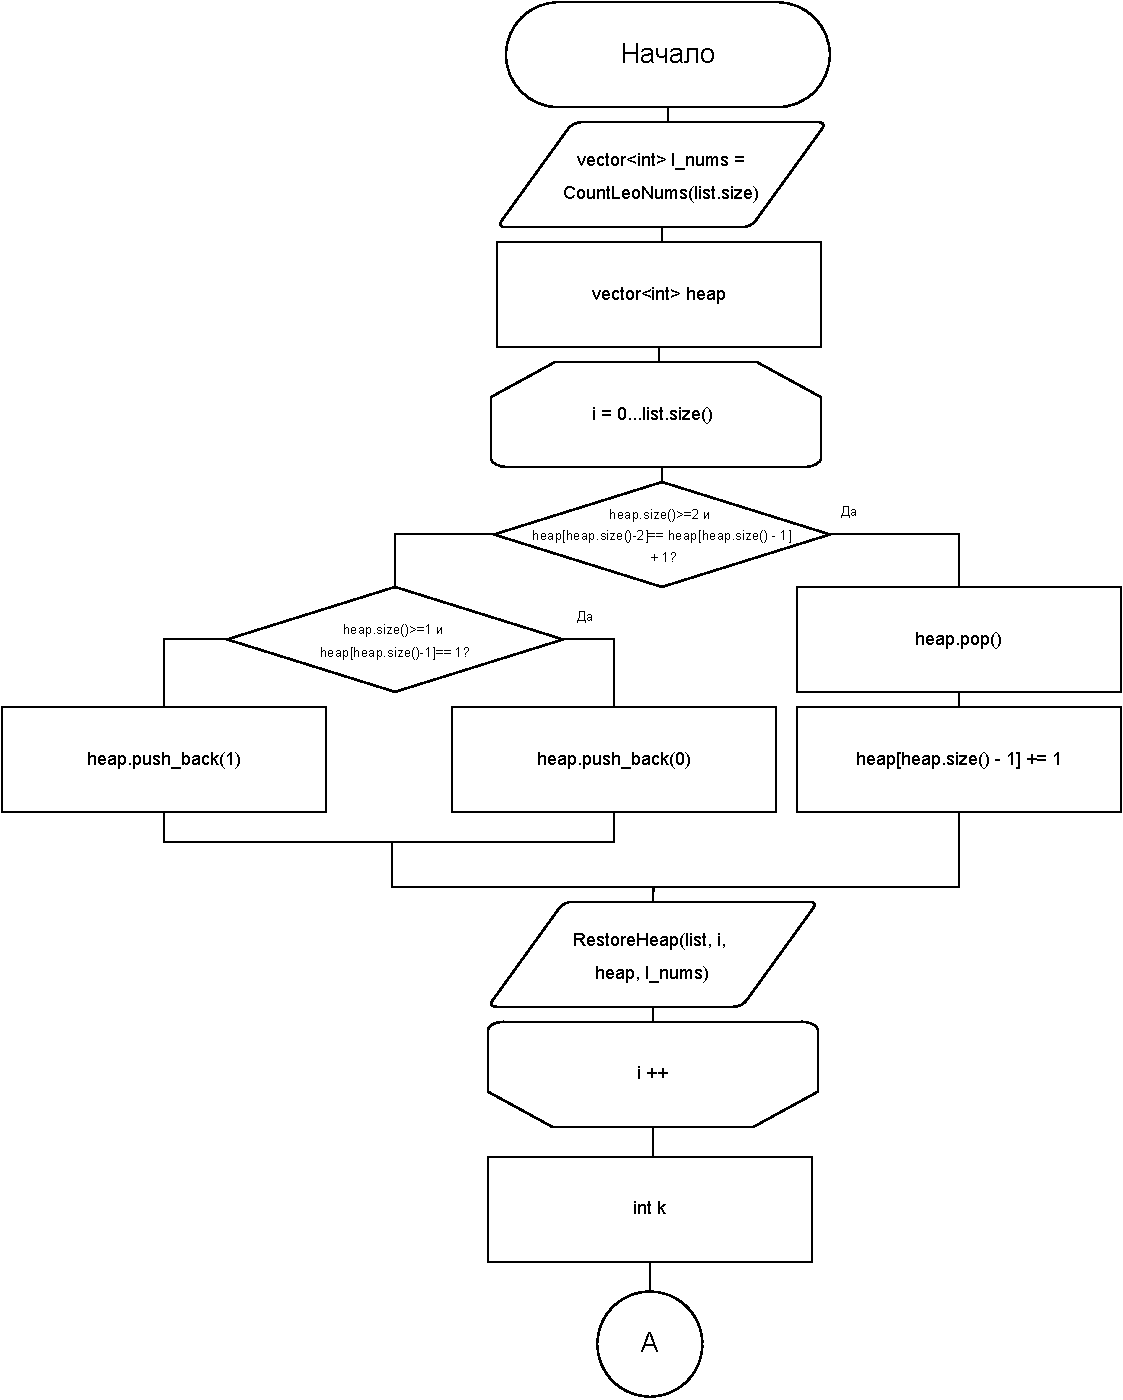
\includegraphics[scale=0.8]{smoothsort.drawio_1.pdf}
       		\caption{Схема плавной сортировки Часть 1}
       		\label{schema:SmoothSort_1}
       	\end{figure}\clearpage
       	
       	\begin{figure}[h!]
            \centering
            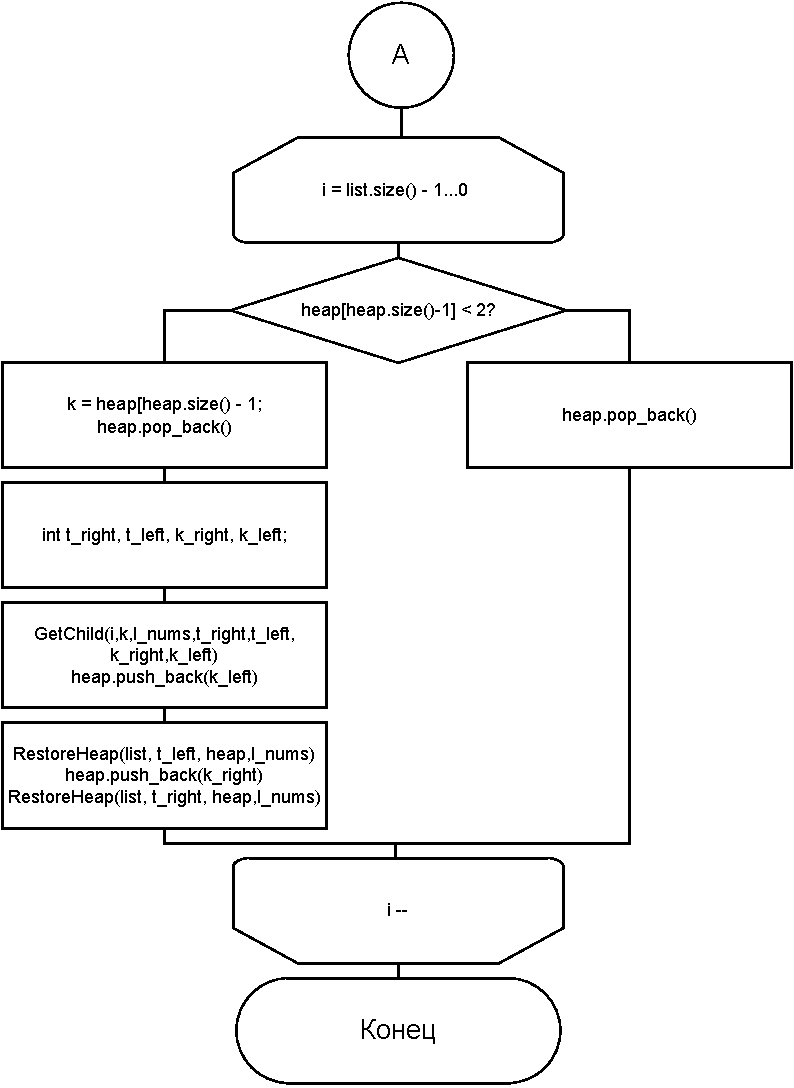
\includegraphics[scale=0.8]{smoothsort.drawio_2.pdf}
            \caption{Схема плавной сортировки Часть 2}
            \label{schema:SmoothSort_2}
        \end{figure}\clearpage

        \begin{figure}[h!]
            \centering
            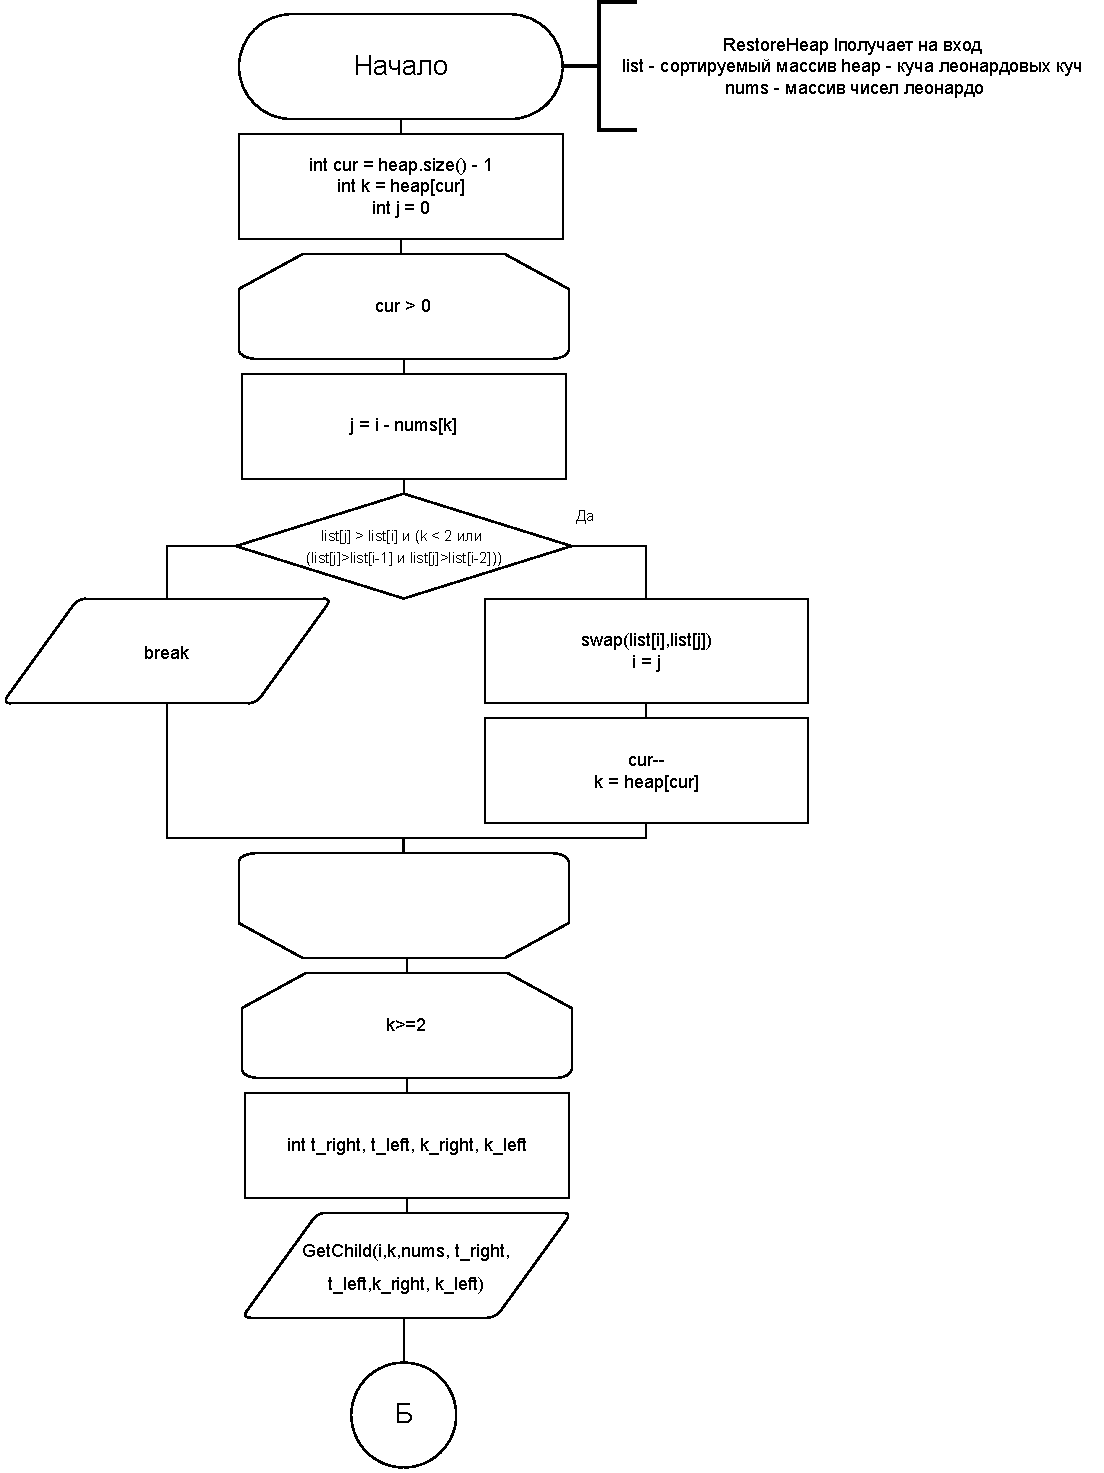
\includegraphics[scale=0.8]{restore_heap_1.pdf}
            \caption{Схема функции RestoreHeap, используемой в плавной сортировке Часть 1}
        \end{figure}\clearpage

        \begin{figure}[h!]
            \centering
            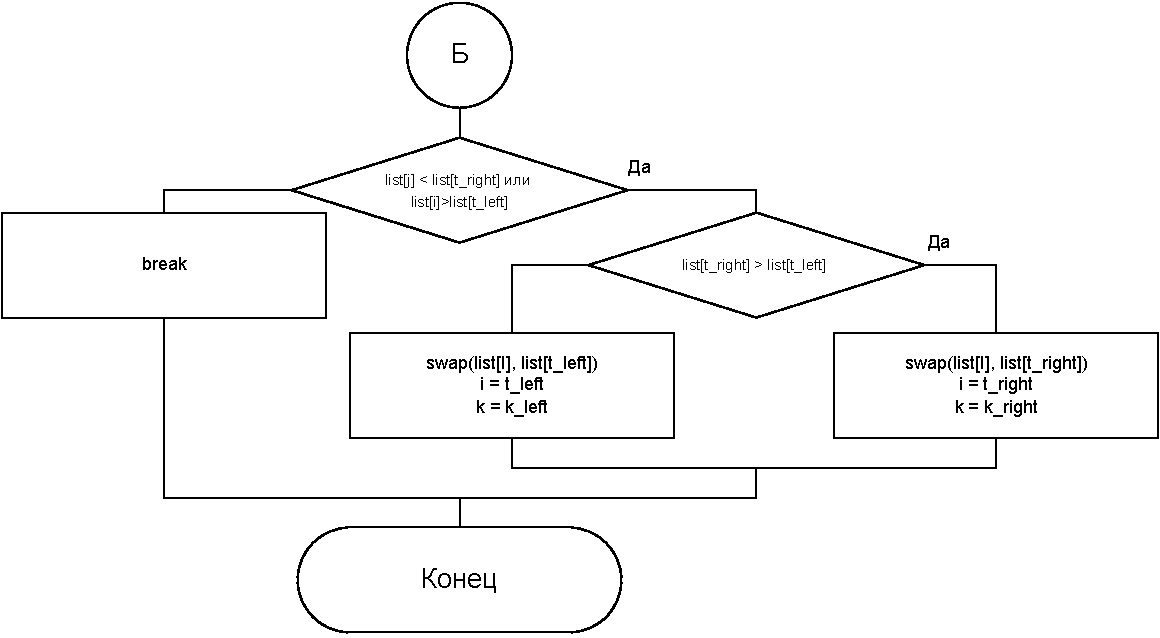
\includegraphics[scale=0.8]{restore_heap_2.pdf}
            \caption{Схема функции RestoreHeap, используемой в плавной сортировке Часть 2}
        \end{figure}\clearpage
        
            \begin{figure}[h!]
            \centering
            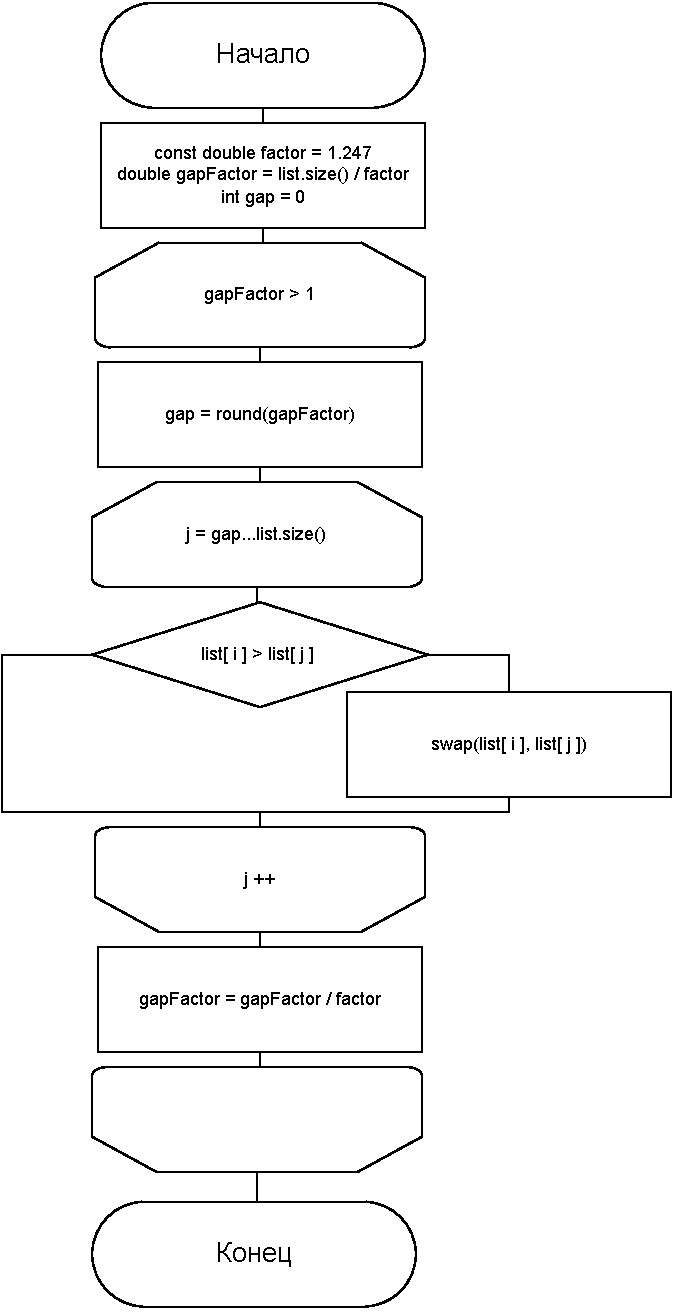
\includegraphics[scale=0.8]{CombSort.pdf}
            \caption{Схема сортировки расчёской}
            \label{schema:CombSort}
        \end{figure}\clearpage

            \begin{figure}[h!]
            \centering
            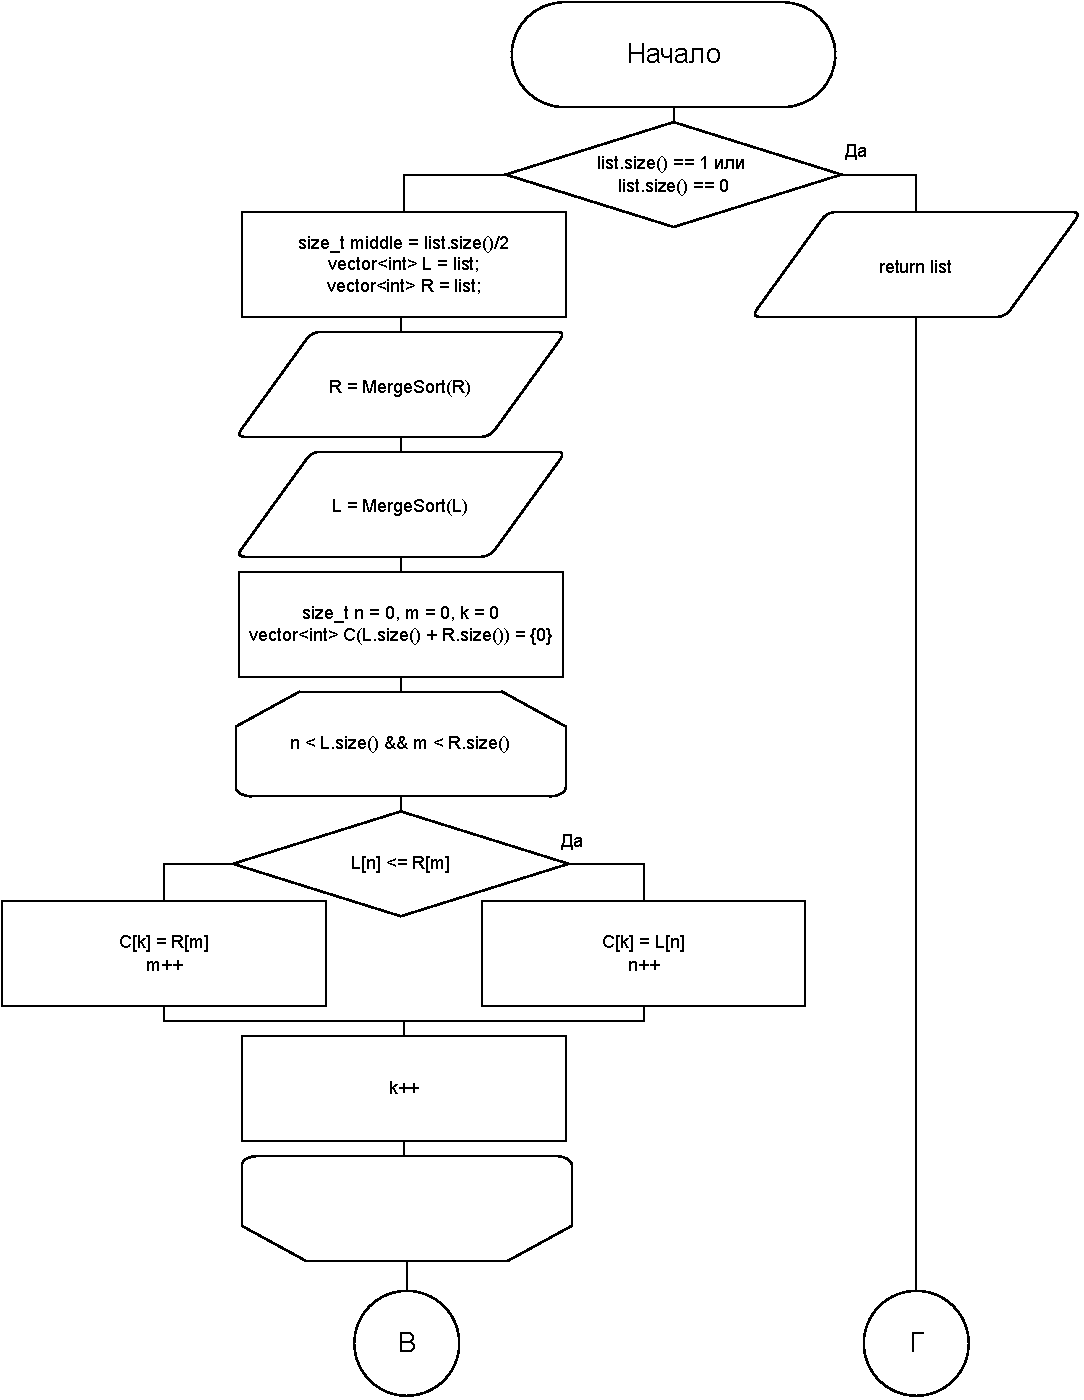
\includegraphics[scale=0.8]{MergeSort_1.pdf}
            \caption{Схема сортировки слиянием Часть 1}
            \label{schema:MergeSort}
        \end{figure}\clearpage

            \begin{figure}[h!]
            \centering
            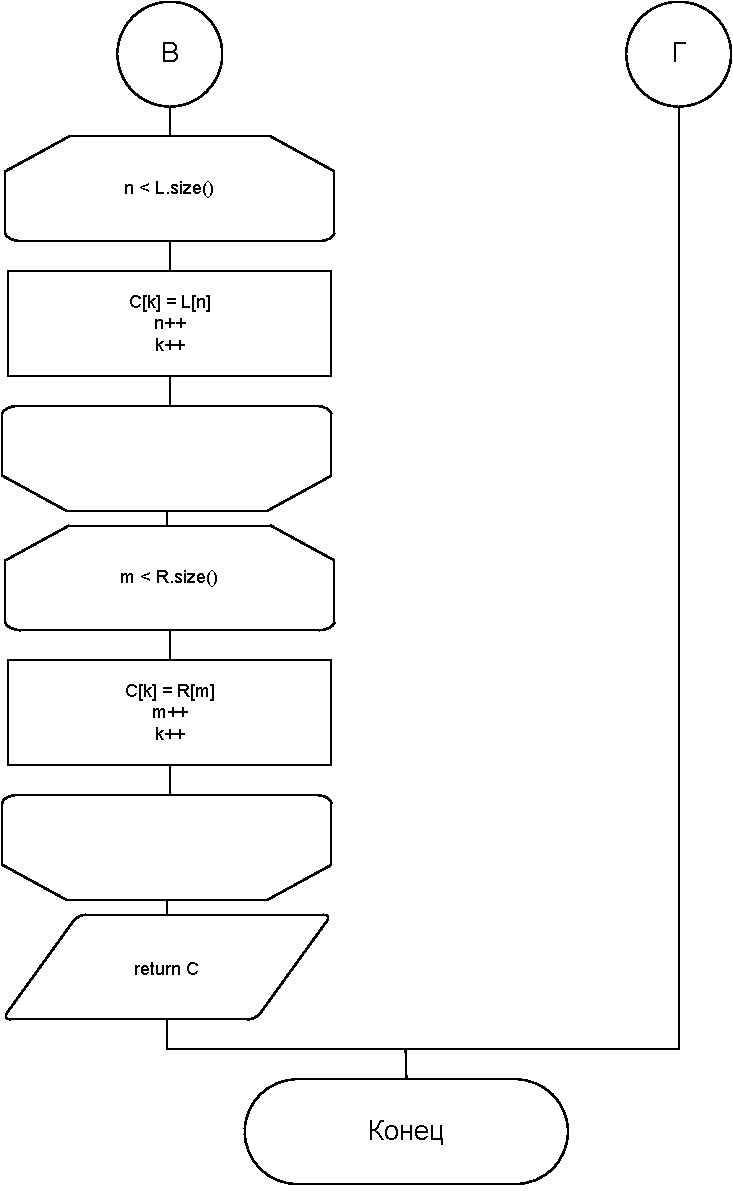
\includegraphics[scale=0.8]{MergeSort_2.pdf}
            \caption{Схема сортировки слиянием Часть 2}
        \end{figure}\clearpage

    \section{Тесты}
    Тестирование ПО будет проводиться методом чёрного ящика. Необходимо проверить работу системы 
    на массивах различной длины.
  	
    \section{Трудоемкость алгоритма}
    \par Трудоёмкость – количество работы, которую алгоритм затрачивает на обработку данных. Является функцией от длины входов алгоритма и позволяет оценить количество работы.
    \par Введём модель вычисления трудоёмкости.

    \subsection{Базовые операции}
    \par Стоимость представленных ниже операций единична:

    \begin{enumerate}
        \item \begin{math} =, +, +=, -, -=, *, *=, /, /=, ++, --, \% \end{math}
        \item \begin{math} <, \leqslant, >, \geqslant, ==, \neq \end{math}
        \item \begin{math} [ ] \end{math}
    \end{enumerate}

    \subsection{Условный оператор}

    \par \begin{math}if(\end{math} условие \begin{math}) \{\end{math}
    \par \begin{math} //\end{math} Тело А
    \par \begin{math}\}\end{math}
    \par \begin{math}else \{\end{math}
    \par \begin{math}//\end{math} Тело В
    \par \begin{math}\}\end{math}
    \par Пусть трудоемкость тела А равна \begin{math}f_A\end{math}, а тела В \begin{math}f_B\end{math}, тогда трудоемкость условного оператора можно найти по формуле (\ref{formula:IfTrud}):

    \begin{equation}\label{formula:IfTrud}
    f_{if} = f_{uslovie} + \begin{cases}
        min(f_A, f_B), &\text{-- лучший случай},\\
        max(f_A, f_B), &\text{-- худший случай}.\\
    \end{cases}
    \end{equation}

    \subsection{Цикл со счетчиком}

    \par \begin{math}for(int\end{math} \begin{math} i = 0; i < n; i++) \{\end{math}
    \par \begin{math} //\end{math} Тело цикла
    \par \begin{math}\}\end{math}

    \par Начальная инициализация цикла \begin{math}int\end{math} \begin{math}i = 0\end{math} выполняется один раз. Условие \begin{math}i < n\end{math} проверяется перед каждой итерацией цикла и при входе в цикл -- \begin{math}n + 1\end{math} операций. Тело цикла выполняется ровно \begin{math}n\end{math} раз. Счётчик \begin{math}i++\end{math} выполняется на каждой итерации, перед проверкой условия, т.е. \begin{math}n\end{math} раз. Тогда, если трудоёмкость тела цикла равна \begin{math}f\end{math}, трудоёмкость всего цикла определяется формулой (\ref{formula:ForTrud}):

    \begin{equation}\label{formula:ForTrud}
    f_{for} = 2 + n(2 + f) 
    \end{equation}

    \subsection{Сортировка расчёской}

    \subsubsection*{Лучший случай}
    \par Массив отсортирован, обмены между элементами не происходят.
    \begin{equation}
    f_{CombSort} = 3 + 1 + M \cdot(1 + 2 + 1 + 3 + N \cdot(3 + 3)) = O(N\cdot \log N)
    \end{equation}

    \subsubsection*{Худший случай}
    \par Массив неотсортирован.
    \begin{equation}
    f_{CombSort} = 3 + 1 + M \cdot(1 + 2 + 1 + 3 + N \cdot(3 + 3 + 3 + 4)) = O(N^2)
    \end{equation}

    \subsection{Сортировка слиянием}

    \subsubsection*{Лучший случай и худший случай}
    \par Так как сортировка происходит в любом случае, то трудоемкость в лучшем и худшем случае одинакова.
    \begin{equation}
    f_{MergeSort} = \frac{N}{2} \cdot (2 + 2 + 2 \cdot N \cdot(2 + 1) + 2 + 3 + 3 + M \cdot (2 + 3 + 4)+ K \cdot(1 + 3 + 2) + L \cdot (1 + 2 + 3)) = O(N\cdot \log N)
    \end{equation}

    \subsection{Плавная сортировка}

    \subsubsection*{Лучший случай}
    \par Массив отсортирован, обмены между элементами не происходят.
    \begin{equation}
    f_{CountLeoNums} = 2 + 2 + N \cdot (1 + 3 + 2) = 4 + N \cdot 6
    \end{equation}
    \begin{equation}
    f_{RestoreHeap} = 2 + 2 + 3 + H_{size} \cdot (2 + 2 + 12) + 1 + M \cdot (1 + 8 + 3 + 3)
    \end{equation}
    \begin{equation}
    f_{SmoothSort} = 1 + f_{CountLeoNums} + 2 + N \cdot (2 + 7 + 3 + f_{RestoreHeap}) + 2 + N \cdot (2 + 3) = O(N)
    \end{equation}

    \subsubsection*{Худший случай}
    \par Массив неотсортирован.
    \begin{equation}
    f_{CountLeoNums} = 2 + 2 + N \cdot (1 + 3 + 2) = 4 + N \cdot 6
    \end{equation}
    \begin{equation}
    f_{RestoreHeap} = 2 + 2 + 3 + H_{size} \cdot (2 + 2 + 12 + 11) + 1 + M \cdot (1 + 8 + 3 + 3 + 3 + 4 + 5)
    \end{equation}
    \begin{equation}
    f_{SmoothSort} = f_{CountLeoNums} + 3 + N \cdot (2 + 7 + 4 + f_{RestoreHeap}) + 2 + N \cdot (16 + 2 \cdot f_{RestoreHeap}) = O(N \cdot \log N)
    \end{equation}

	\section*{Вывод}
    \par Сортировка расчёской: лучший -- \begin{math}O(N\cdot \log N)\end{math}, худший -- \begin{math}O(N^2)\end{math}.
    \par Сортировка слиянием: лучший -- \begin{math}O(N\cdot \log N)\end{math}, худший -- \begin{math}O(N\cdot \log N)\end{math}.
    \par Плавная сортировка: лучший -- \begin{math}O(N)\end{math}, худший -- \begin{math}O(N\cdot \log N)\end{math}.
\newpage